\documentclass[12pt]{article}
\usepackage{graphicx}
\usepackage{xcolor}
% \usepackage[margin=1.7cm]{geometry}
\usepackage{colortbl}
\usepackage{tikz}
\usepackage{amsmath}
\usepackage{caption}
\usepackage{subcaption}
\begin{document}
\begin{titlepage}
\begin{center}
    
\includegraphics[width=\textwidth]{./logo.png}
    \\ [2.5cm]
    \textsc{\Large Autonomous Mobile Robots}
    \\ [0.5cm]
    \textsc{\large First assignment}
    \\ [1cm]
    \hrule
    \vspace{0.3cm}
    \textsc{OpenLoop Steering Assignment}
    \\ [0.3cm]
    \hrule
    \vfill
    \textsc{Ruben Janssen, 10252657 \\ David van Erkelens, 10264019 \\ Laurens Verspeek, 10184465 \\[0.7cm] Department of Computer Science \\ University of Amsterdam \\[0.3cm] \today}
\end{center}
\end{titlepage}
\tableofcontents
\clearpage
\section{Introduction}
In this report the first findings of programming the NXT to follow a certain path given by circles and lines will be described. 
\section{Kinematic Models}
The following formula is given: 
\begin{equation}
    \begin{bmatrix} 
        \dot{x} \\ 
        \dot{y} \\ 
        \dot{\theta}
    \end{bmatrix} 
    = f(\dot{\varphi_1}, \dot{\varphi_2}, l, r, l_c, d, r_c, \ldots)
    \label{start}
\end{equation}
When applying this to the differential drive robot, $r$ denotes the diameter of the wheels and $l$ denotes the distance between the origin of the robot and the wheels. A $l$ and $r$ with an underscore $c$ denotes these distances for the castor wheel. The $d$ denotes the distance between the wheel contact point and the center of rotation of the castor wheel. $\varphi_1$ and $\varphi_2$ denote the movement of the wheels. In figure \ref{wheels}, the allocation of $\varphi_1$ and $\varphi_2$ to the wheels is shown. In case of the omni-drive robot, $\varphi_n$ denotes the movement of the $n^{th}$ wheel and $l$ and $r$ have the same meaning as with the differential-drive robot.
\begin{figure}[h!]
    \centering
    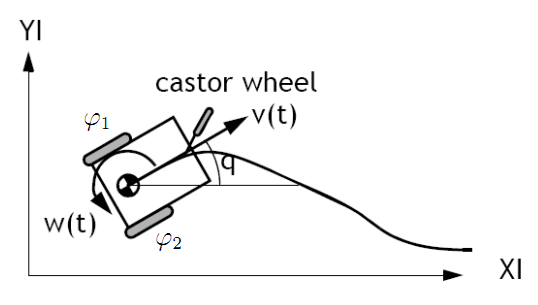
\includegraphics[width=0.5\textwidth]{wheels.png}
    \caption{The allocation of $\varphi_1$ and $\varphi_2$}
    \label{wheels}
\end{figure}
\clearpage
\subsection{Establishing the kinematics}
Moving onwards with formula \ref{start}, we can establish the kinematics of the differential-drive robot (shown in formula \ref{for:div}) and the omni-drive robot (shown in formula \ref{for:omni}).
\begin{equation}
    \begin{bmatrix} 
        \dot{x} \\ 
        \dot{y} \\ 
        \dot{\theta}
    \end{bmatrix} 
    = f(l, r, \dot{\varphi_1}, \dot{\varphi_2})
    \label{for:div}
\end{equation} 
\begin{equation}
    \begin{bmatrix} 
        \dot{x} \\ 
        \dot{y} \\ 
        \dot{\theta}
    \end{bmatrix} 
    = f(l, r, \dot{\varphi_1}, \dot{\varphi_2}, \dot{\varphi_3})
    \label{for:omni}
\end{equation} 
In the formula for the differential drive robot, $l_c$ is left out since the influence of the castor wheel on the movement is negligible.
\subsubsection{Odometry of differential drive robot}
\paragraph{a} \begin{equation}
\xi_I = 
\begin{bmatrix} \dot{x} \\ \dot{y} \\ \dot{\theta} \end{bmatrix}
= 
\begin{bmatrix} \cos \theta && - \sin \theta && 0 \\
\sin \theta && \cos \theta && 0 \\
0 && 0 && 1 \end{bmatrix} 
\begin{bmatrix} \frac{r\dot{\varphi_1}}{2} + \frac{r\dot{\varphi_2}}{2} && 0 \\ 0 && 1 \\ \frac{r\dot{\varphi_1}}{2l} + \frac{-r\dot{\varphi_2}}{2l} && 0\end{bmatrix}
\end{equation}

Als je de matrix invult, wordt \theta ingevuld met \omega. y is altijd 0 want je rijdt in x richting. x is de afstand in meters/whatever.

\paragraph{b} The larger ${\Delta}t$, the less precise the estimation of the position is. The rotation $w$ increases when the difference between $\varphi_1$ and $\varphi_2$ increases ($\varphi_1$ and $\varphi_2$ are the speed of the wheels). The heading speed $v$ increases when the sum of $\varphi_1$ and $\varphi_2$ increases.
\clearpage
\section{Preparation for a real experiment}
\paragraph{a} First, the circle to be followed has to be determined, using a radius $r$. Then, the number of degrees to follow the circle should be determined, as $g$. \\ 
To move the robot as desired, the distance to travel with each wheel should be calculated. 
\begin{equation}
\begin{split}
    D_1(r) = 2\pi \times (r - l) \\
    D_2(r) = 2\pi \times (r + l)
\end{split}
\end{equation}
In which $D_1$ notes the wheel closest to the center of the circle, and $D_2$ the wheel farthest from the center of the circle. Now the number of rotations to travel this distance should be calculated. This is done by dividing by the diameter $d$ of the wheels:
\begin{equation}
\begin{split}
    Rotations_1(r) = \frac{D_1(r)}{d_{wheel}} \\
    Rotations_2(r) = \frac{D_2(r)}{d_{wheel}}
\end{split}
\end{equation}
The speed of the wheel closest to the center of the circle will be lowered, so $\frac{\varphi_1}{\varphi_2} = \frac{Rotations_1(r)}{Rotations_2(r)}$. Then, $\varphi_1$ will become $\varphi_1 \times \frac{Rotations_1(r)}{Rotations_2(r)}$. After this, the \verb|Tacho|-limit of the of the wheels will be set to the values of $Rotations_1(r)$ and $Rotations_2(r)$. Since $\frac{\varphi_1}{\varphi_2} = \frac{Rotations_1(r)}{Rotations_2(r)}$, both wheels will finish their rotations on the same moment. \\ \\
To make the robot drive in a straight line, only the \verb|Tacho|-limit is of importance. The \verb|Tacho|-limit can be defined as a function $f$ in a distance to travel $t$:
\begin{equation}
    f_n(t) = 360 \times Rotations_n(r)
\end{equation}
\paragraph{b} In order to implement a feedback-loop, the \verb|Tacho|-limit is removed. Instead, every 0.1 the value of both wheels is read to check if they already meet the value which would have been the \verb|Tacho|-limit. If the values are incorrect, movement is reversed or continued. If the read value equals the desired regarding a certain threshold, movement of the wheel is stopped.
\paragraph{c} For the Matlab implementation, see \verb|circle.m|, \verb|straightLine.m|, \verb|drive.m| and \verb|henk.m| (named after the robot).
\clearpage
\section{Experiments}
In order to test the code and formulas, the robot was tested in the \textit{Robolab}. In the \textit{Robolab} lies a football field used for Naos, but that field was perfectly suitable for testing our NXT. The NXT was programmed to follow the circle in the center of the field, which has a diameter of 60cm. In figure \ref{driveline}, the path of the NXT across this line is shown. On the pictures the NXT has a small offset from the line, but this can be explained by a faulty starting position. \\
\begin{figure}[h!]
    \centering
    \begin{subfigure}[b]{0.3\textwidth}
            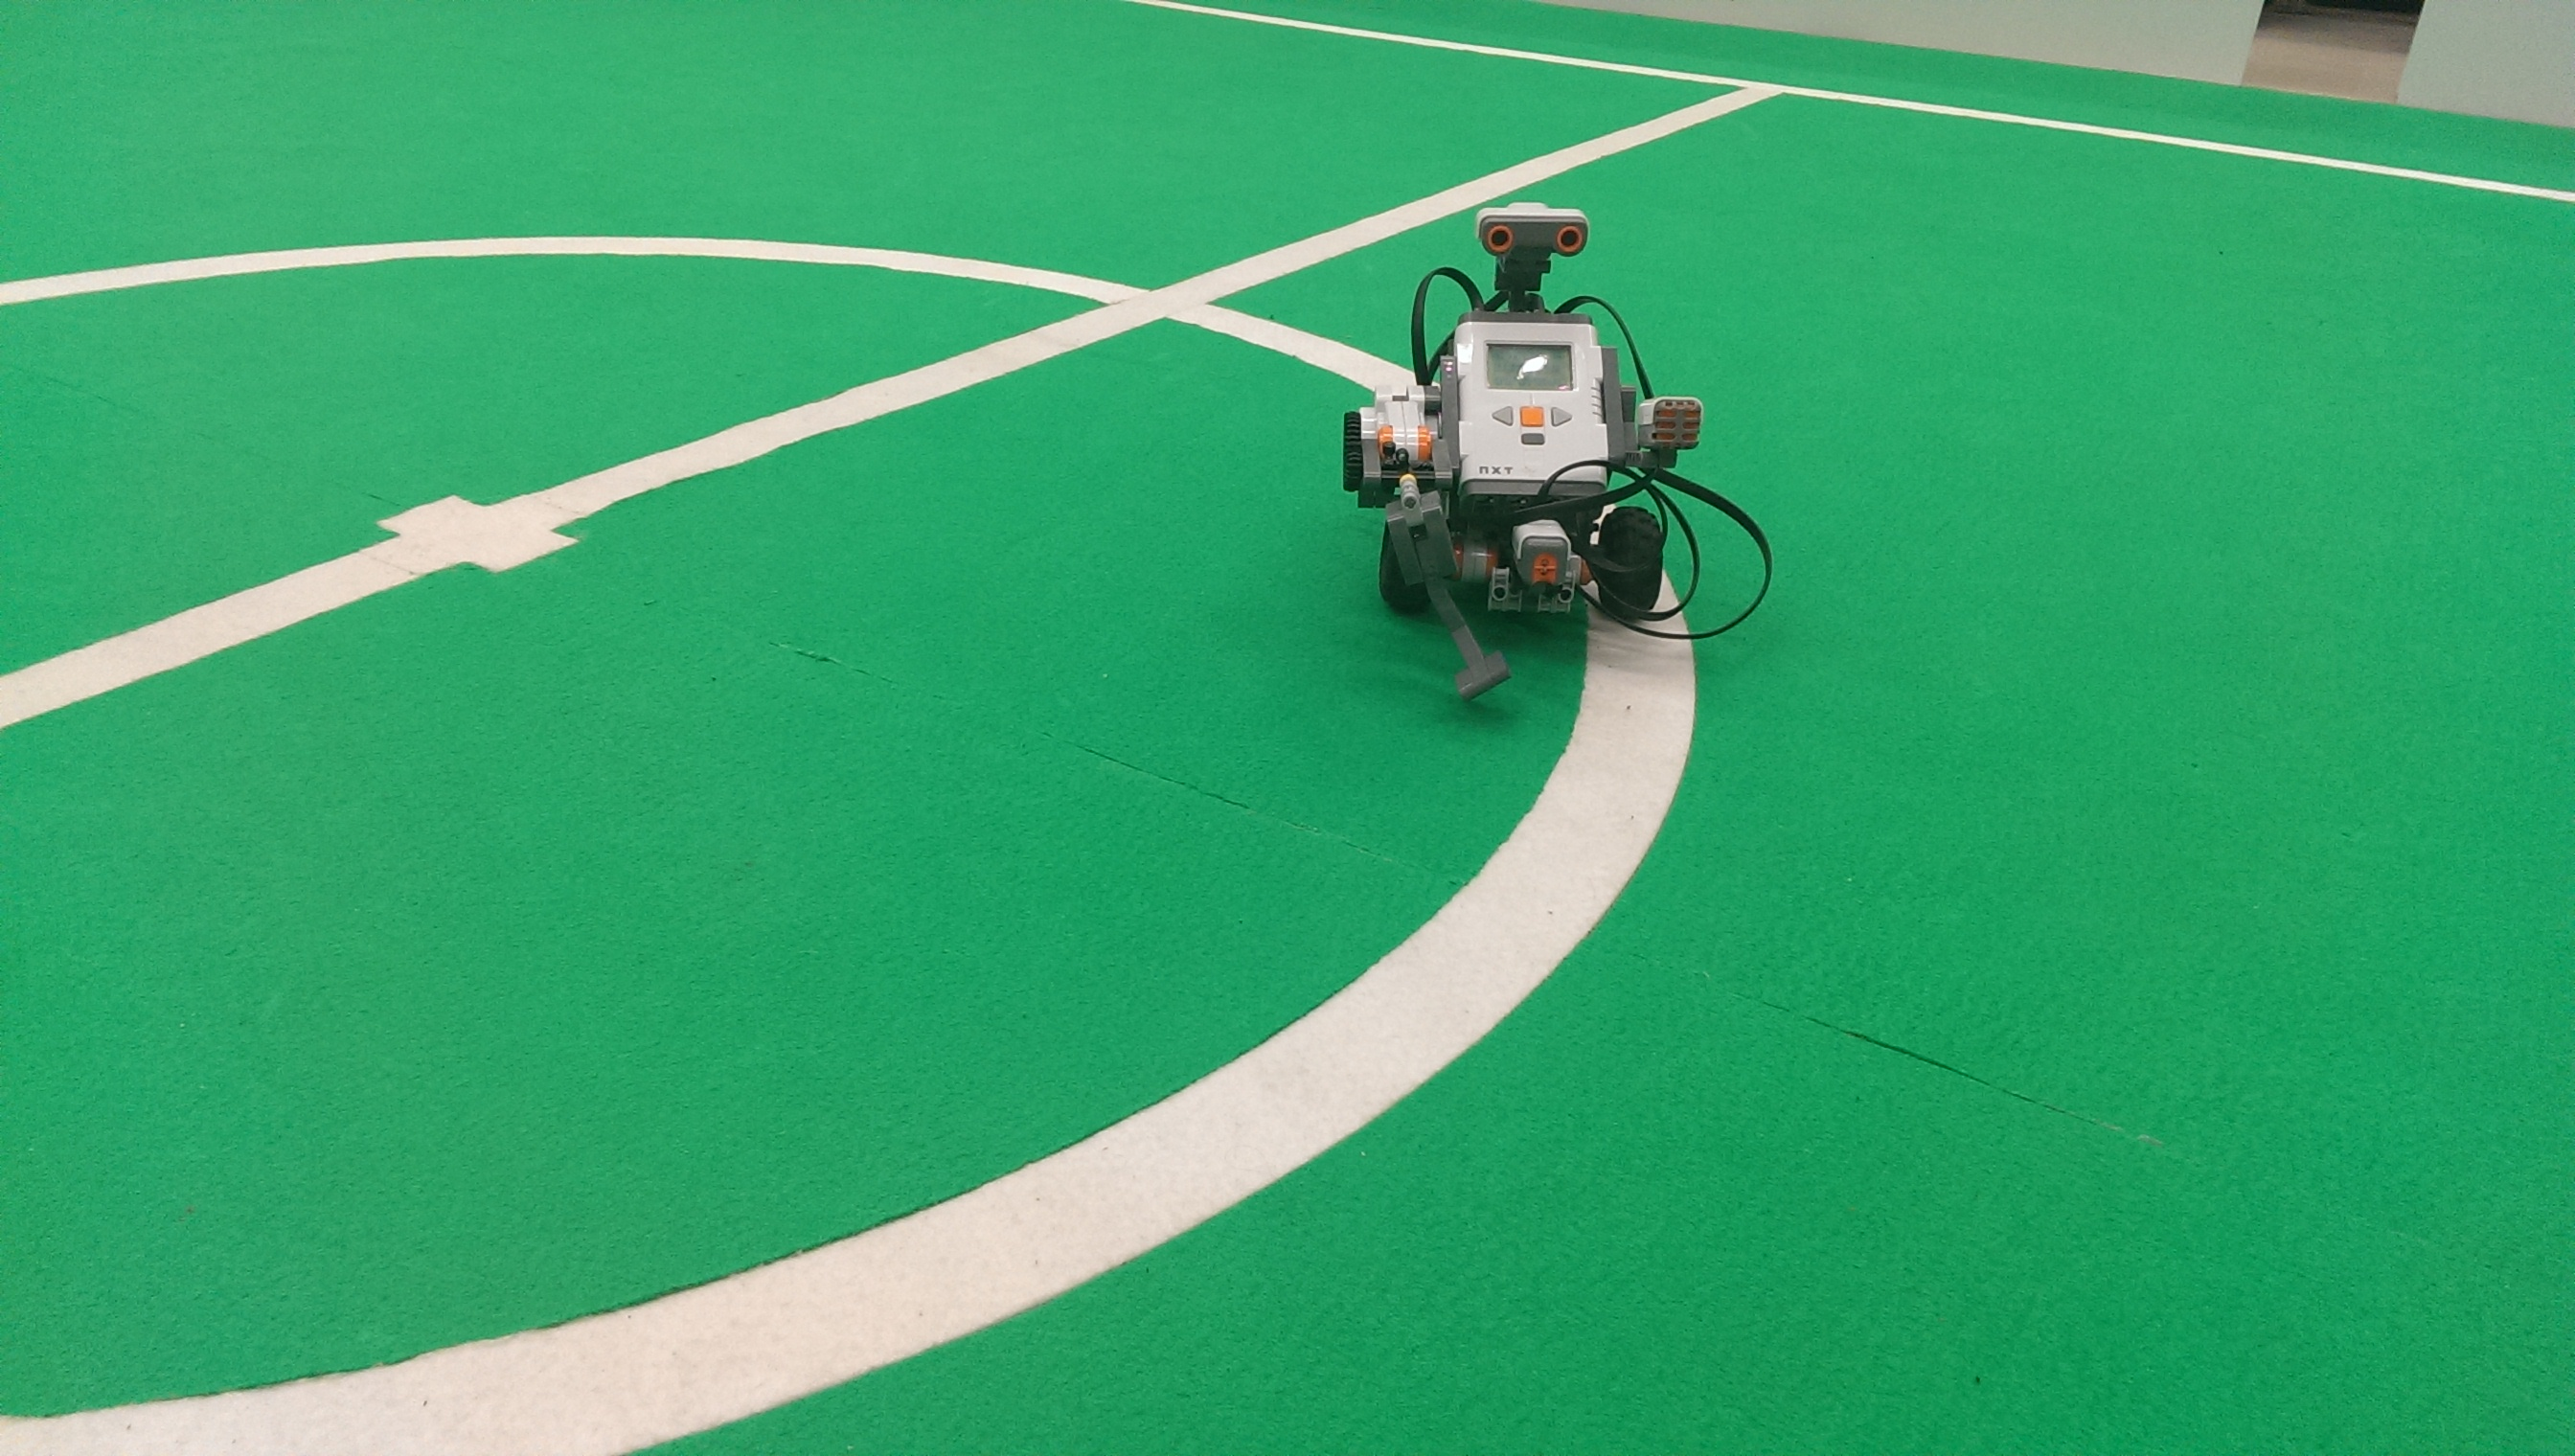
\includegraphics[width=\textwidth]{lijn1.jpg}
    \end{subfigure}%
    ~ 
    \begin{subfigure}[b]{0.3\textwidth}
            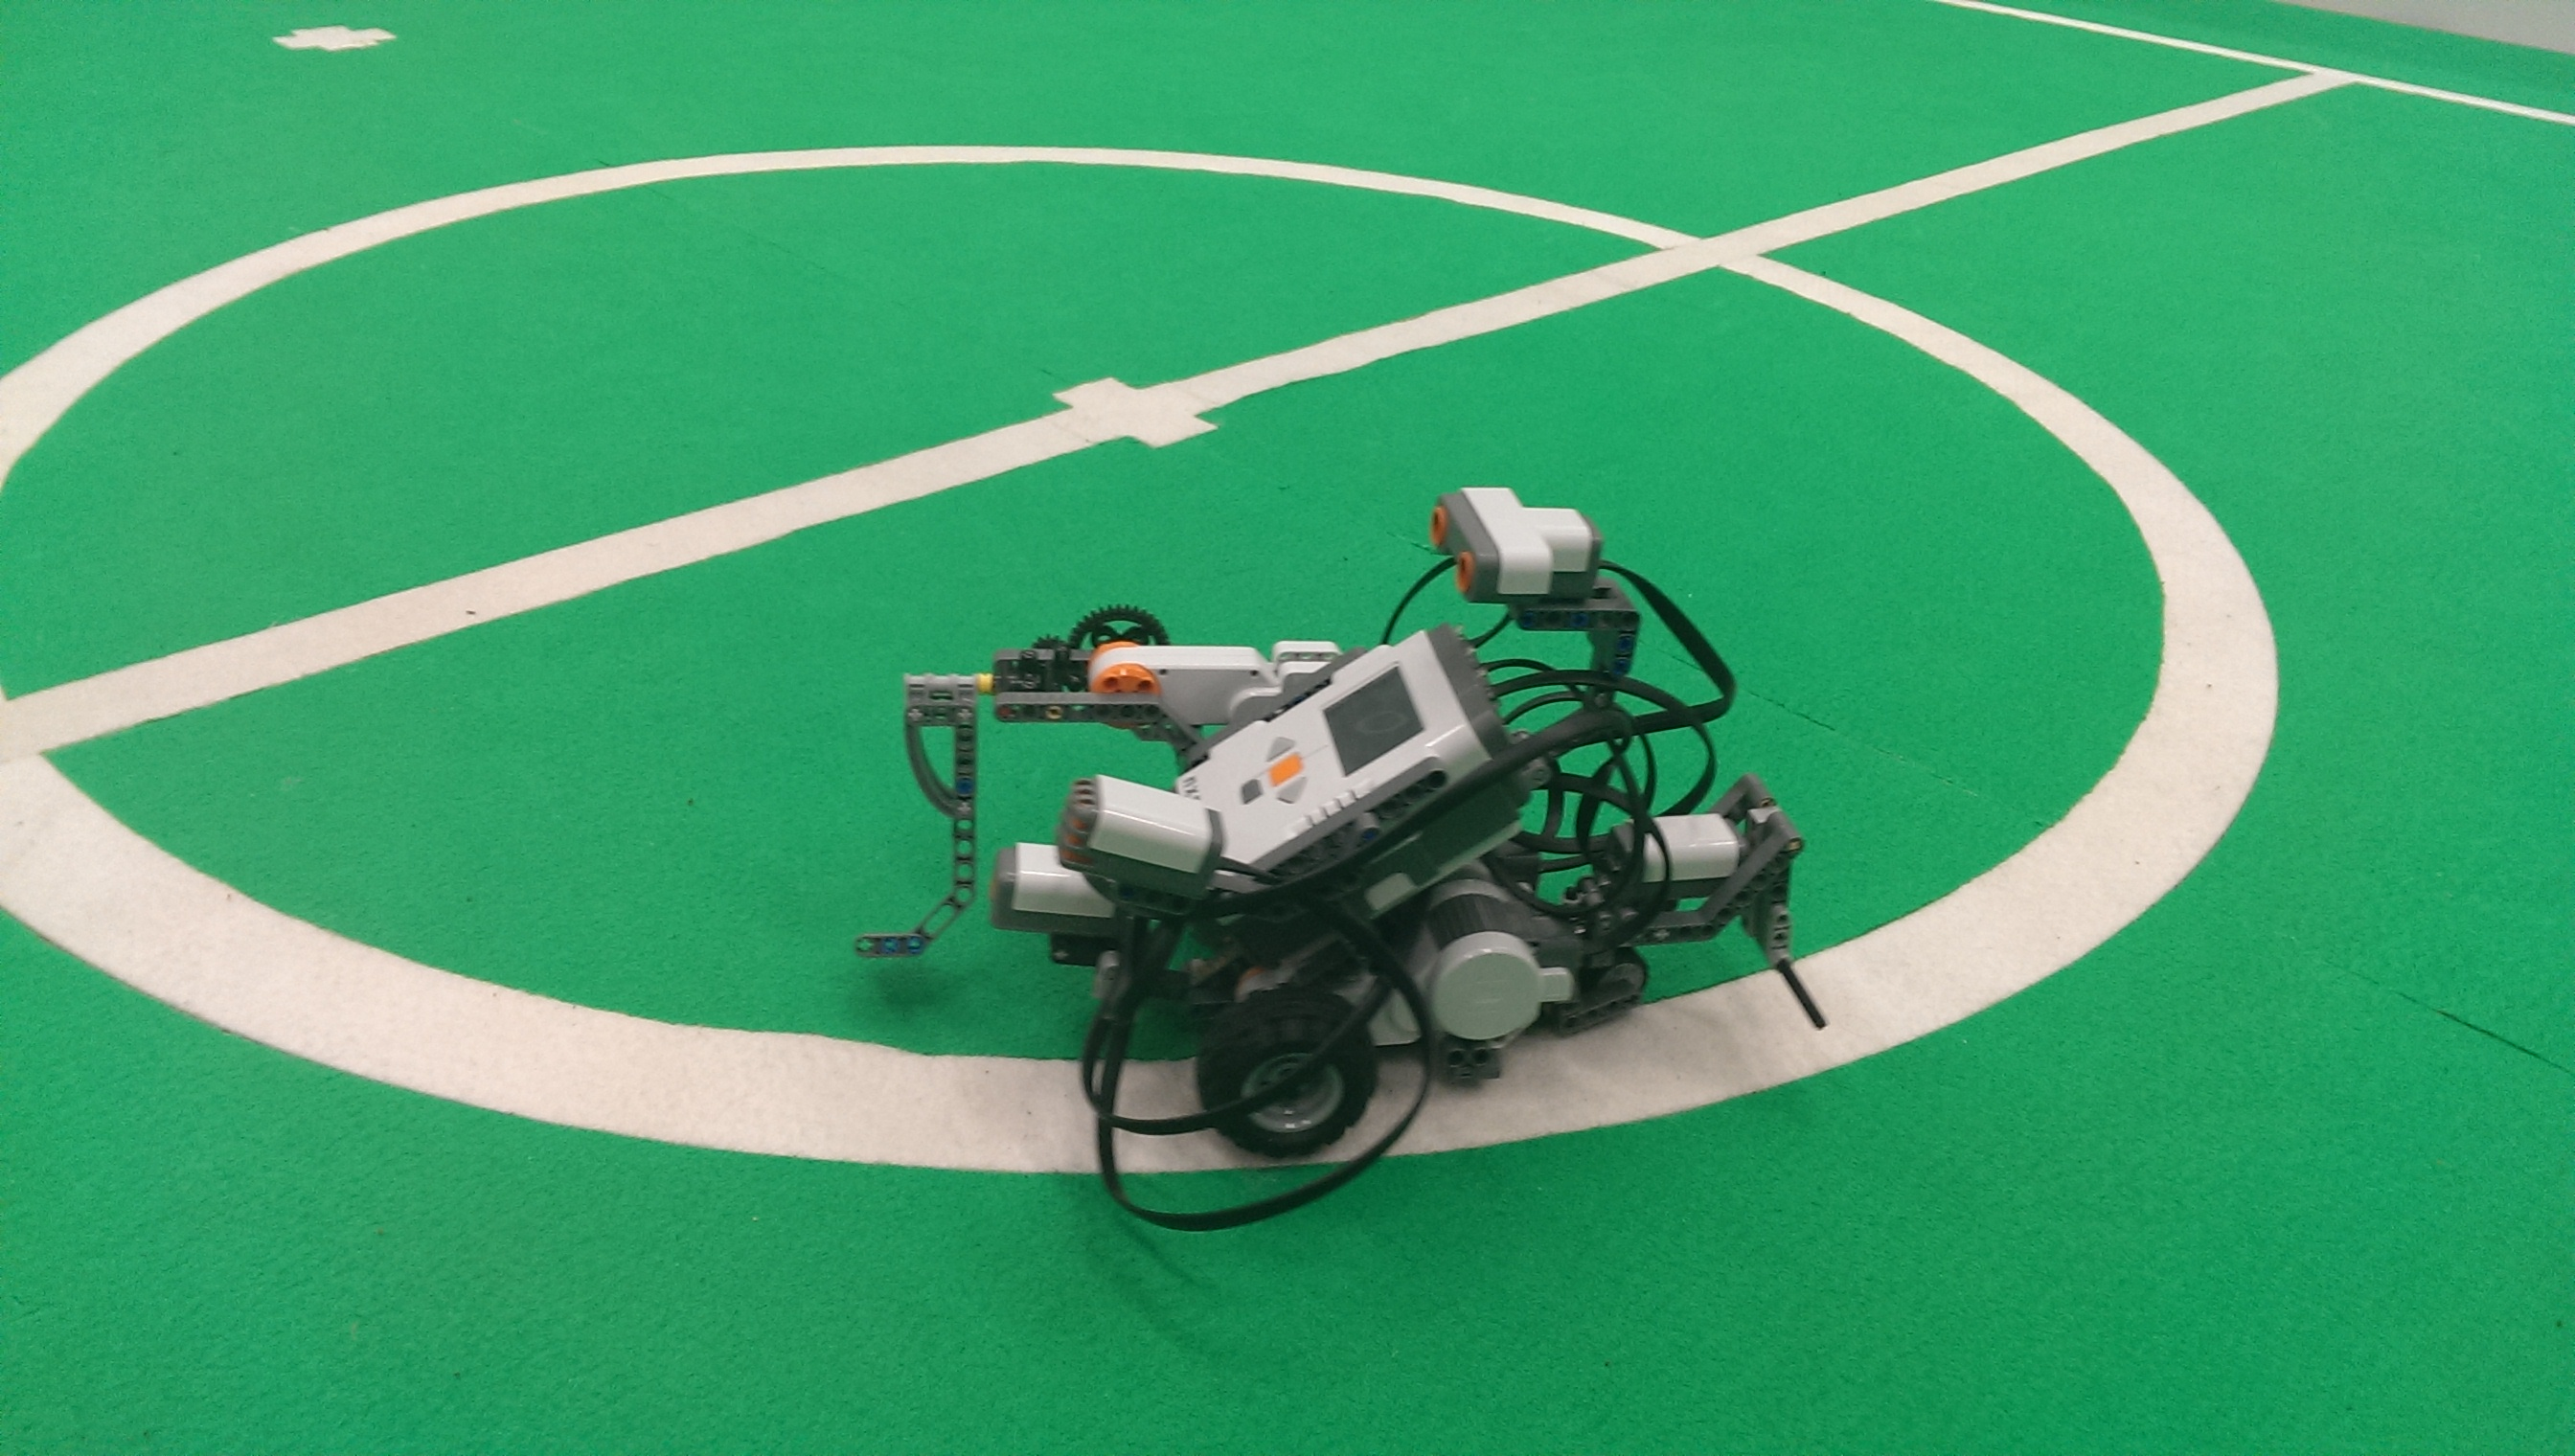
\includegraphics[width=\textwidth]{lijn2.jpg}
    \end{subfigure}
    ~ 
    \begin{subfigure}[b]{0.3\textwidth}
            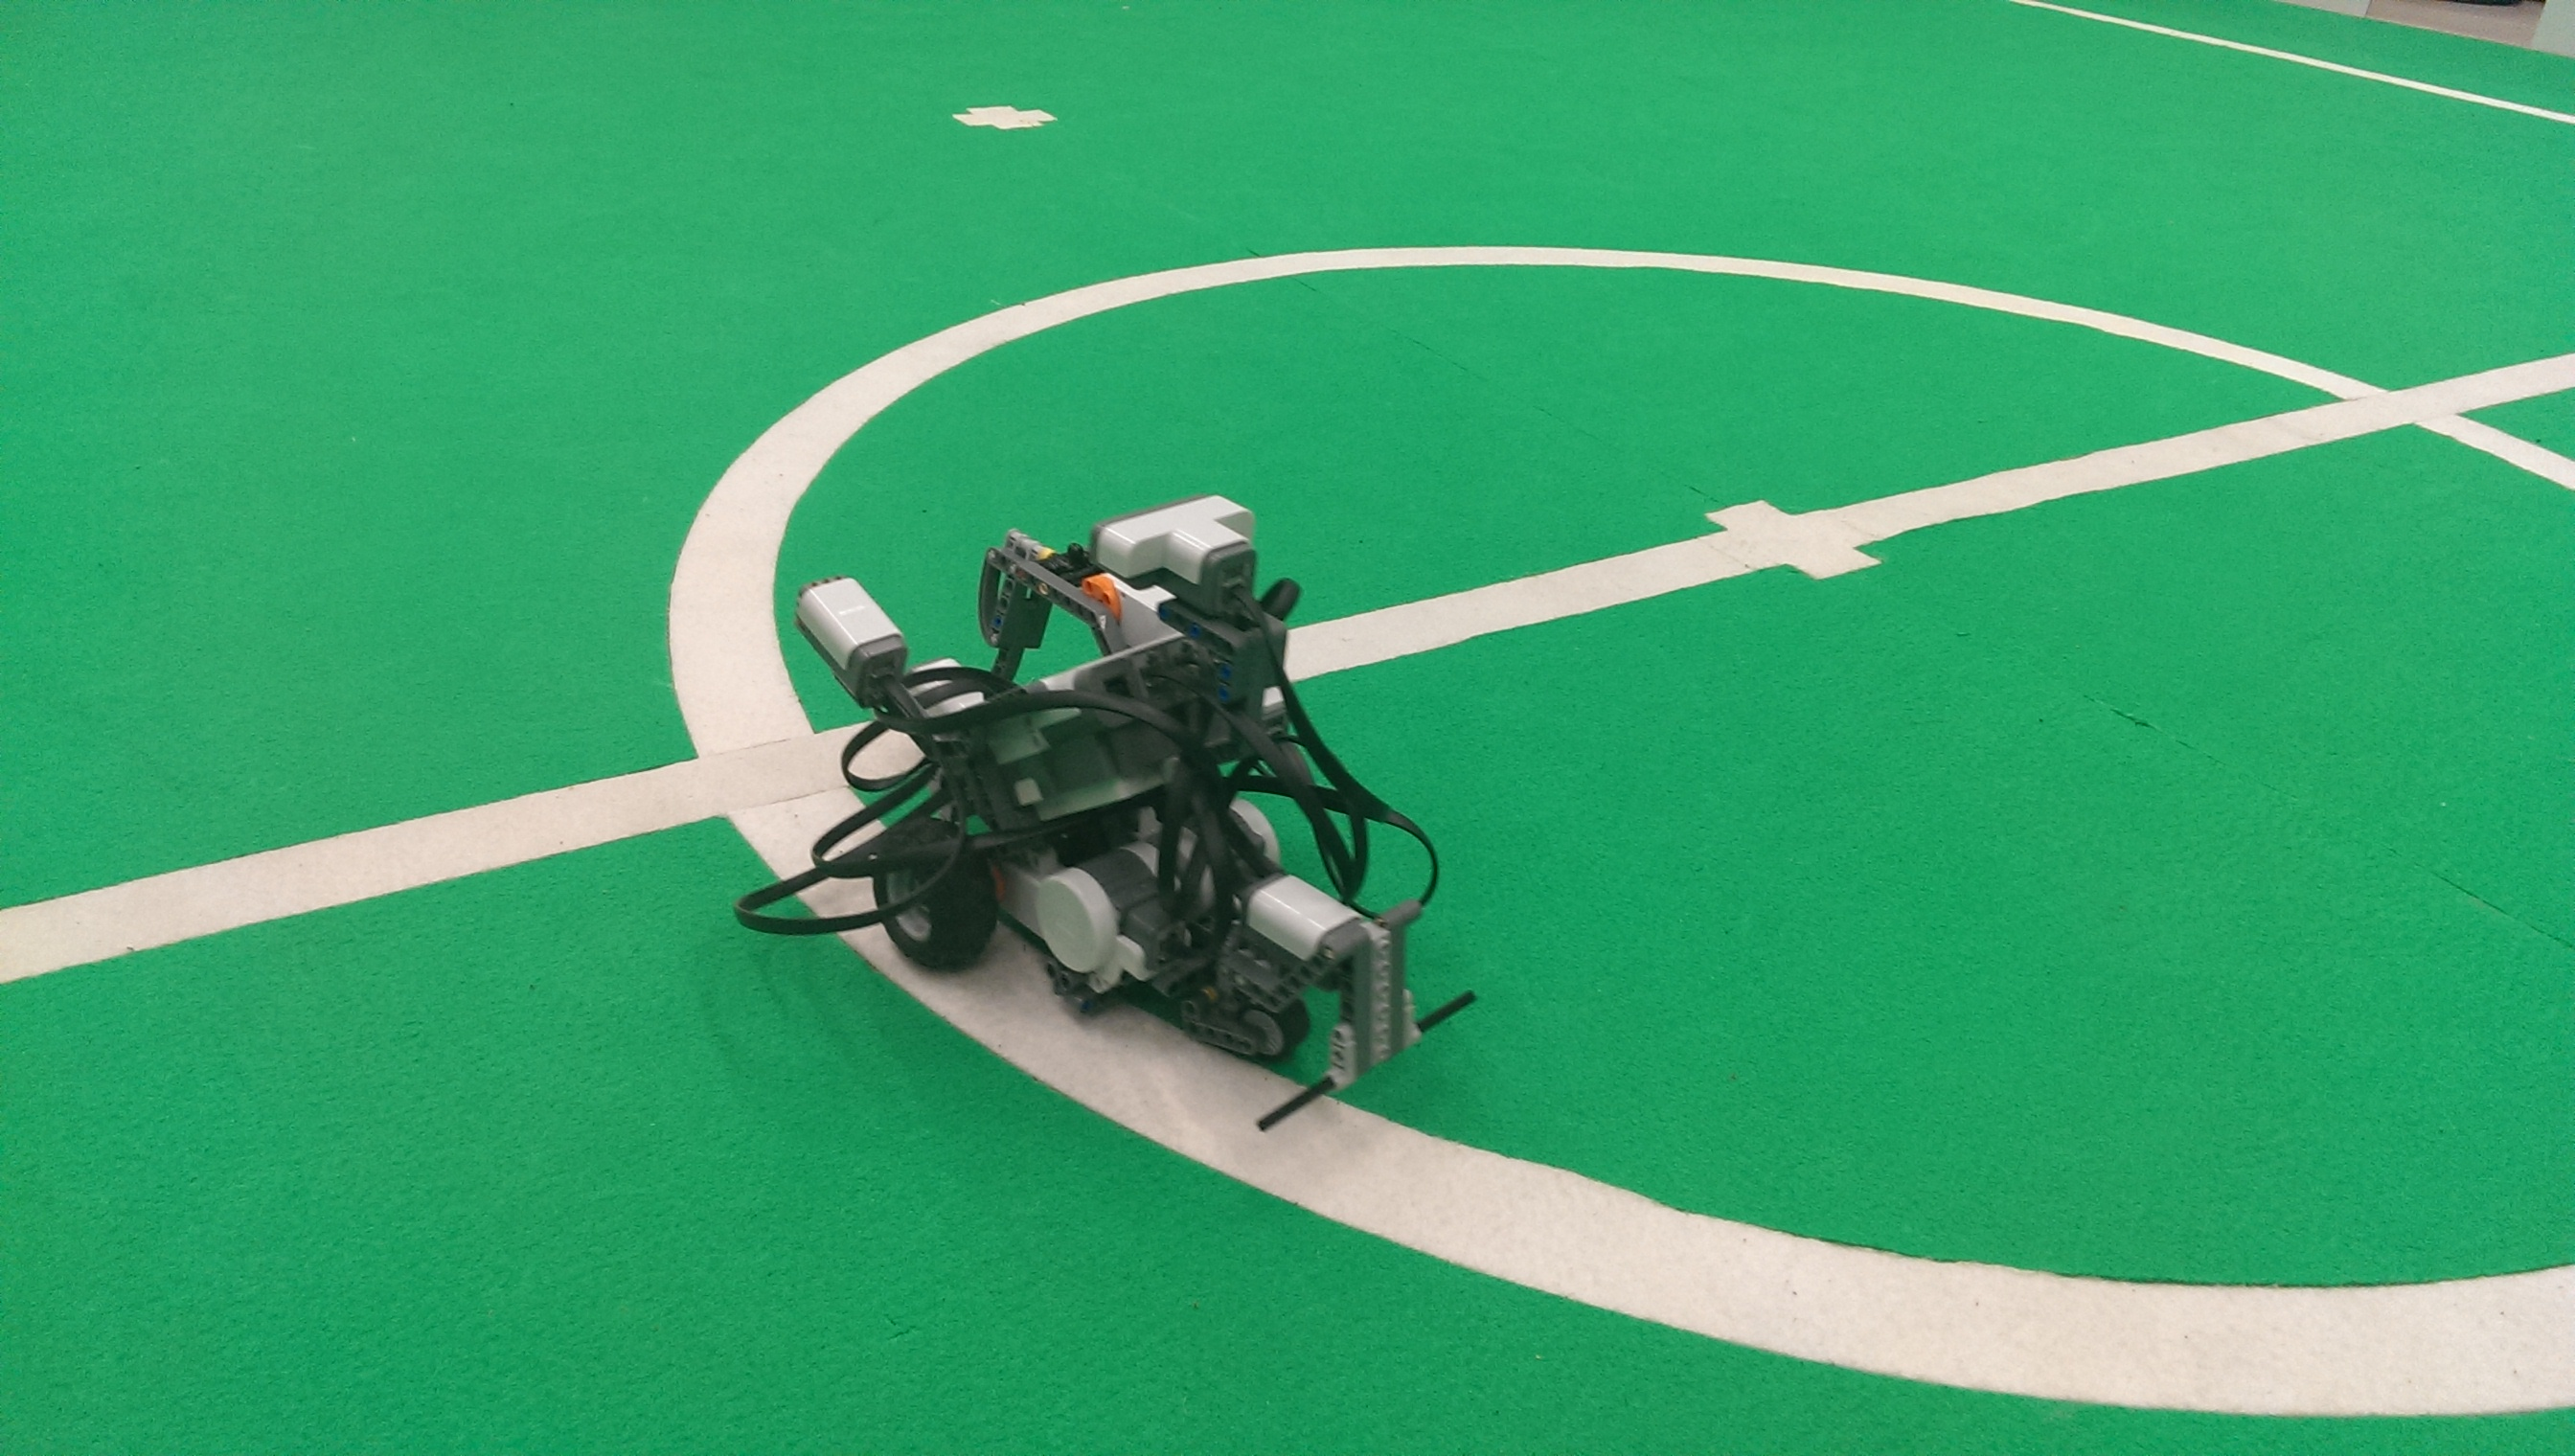
\includegraphics[width=\textwidth]{lijn3.jpg}
    \end{subfigure}
    \caption{The NXT driving along the line}
    \label{driveline}
\end{figure}
\section{Conclusions}
Looking at the experiments, it can be concluded that the formulas and code function, because the NXT was able to follow the line on the field pretty closely.
\end {document}